\documentclass[sigconf]{acmart}

\usepackage[linesnumbered,ruled]{algorithm2e}
\usepackage{listings}

%Defining Colors used by listing package
\definecolor{mygray}{rgb}{0.5,0.5,0.5}
\definecolor{mygreen}{rgb}{0,0.6,0}
\definecolor{mymauve}{rgb}{0.58,0,0.82}

\lstset{ breaklines=true,
basicstyle=\footnotesize,
numbers=left,
frame=single,
showstringspaces=falsebasicstyle=\ttfamily,
keywordstyle=\color{blue}\ttfamily,
stringstyle=\color{red}\ttfamily,
commentstyle=\color{green}\ttfamily,
morecomment=[l][\color{magenta}]{\#}}

\renewcommand{\lstlistingname}{Code Snippet}% Listing -> Algorithm
\renewcommand{\lstlistlistingname}{List of \lstlistingname s}% List of Listings -> List of Algorithms

\AtBeginDocument{%
  \providecommand\BibTeX{{%
    \normalfont B\kern-0.5em{\scshape i\kern-0.25em b}\kern-0.8em\TeX}}}

\setcopyright{acmcopyright}
\copyrightyear{2018}
\acmYear{2018}
\acmDOI{10.1145/1122445.1122456}

\acmConference[CS6161]{UVA '19: CS6161 - Compilers}{December 06, 2019}{Charlottesville, VA}
\acmBooktitle{UVA '19: CS6161 - Compilers,
  December 06, 2019, Charlottesville, VA}
\acmPrice{0.00}
\acmISBN{978-1-4503-9999-9/18/06}

\begin{document}
\title{Compilers Final Project - Concolic Testing in LLVM }

\author{Carl Hildebrandt}
\affiliation{\institution{The University of Virginia}}
\email{ch6wd@virginia.edu}

\author{Will Leeson}
\affiliation{\institution{The University of Virginia}}
\email{wel2vw@virginia.edu}

\newcommand{\CH}[1]{{\color{red}CH: #1}}
\newcommand{\WL}[1]{{\color{blue}WL: #1}}

\begin{abstract}
  Concolic Execution is a testing strategy that utilizes both concrete
  testing and symbolic execution to make up for the shortcomings of each
  technique. Concrete execution is as fast as the program in question. 
  However, if inputs are being generated at random, it may take far
  too many tests to satisfy all paths of execution. Symbolic execution 
  can find all paths of execution. However, this can be computationally 
  expensive. Concolic execution leverages one against the other. Symbolic 
  execution can find the paths in which concrete testing has difficulty
  reaching. Concrete execution can execute the hard to solve paths. Many
  concolic execution tools target a specific language. This can lead to
  time spent re-targeting tools to other languages. LLVM is a compiler
  infrastructure that allows for creation of compilers that produce 
  the same intermediate representation, LLVM bitcode. In this paper, we 
  design a concolic execution strategy that can be used on LLVM bitcode.
  This will allow for a concolic execution tool that can be used on
  languages that can be compiled into LLVM bitcode.
\end{abstract}

\keywords{Concolic Execution, LLVM, Static Analysis, Dynamic Analysis, Compilers}

\maketitle

\section{Introduction}

Symbolic execution and concrete execution are two testing techniques
that can be used to find and test execution paths through a program.
Symbolic execution finds the constraints of a program to discover paths
of through the program. In order to test these paths, it generates the constraints
that need to be satisfied to execute it. It then passes these constraints
to a tool, like the SMT solver Z3 \cite{10.1007/978-3-540-78800-3_24}, which
decides if these constraints are satisfiable. If it is satisfiable, it can model
this solution with a input that with execute the path in question. Solving
these constraints can quickly become difficult as the constraints become
more and more complex. As a result, using symbolic execution tools can become
infeasible with complex programs. 

On the other end of the spectrum, there is concrete execution. Unlike symbolic
execution, concrete execution is relatively inexpensive. The test is as 
expensive as the program in question. This allows
for running many tests to exercise as many paths as possible. Often the input
for automated concrete execution is randomly generated. If the probability of
going down any path is fairly uniform, testing all paths is fairly simple. 
However, if the probability of hitting certain paths is low, it can be 
difficult to exercise all paths. However if combined correctly, these tools
can compliment each other resulting in a more accurate yet cheap automated test tool. 

Another issue common in many software testing tools is that the tool can only 
target a specific language. This can lead to several tools that may 
accomplish the same task, only for different targets. The scope of the 
tool can be expanded if it targets a more general language. LLVM is
a compiler infrastructure that provides the tools for developers to
make compilers for their own languages or existing languages. LLVM
compilers produce an intermediate representation known as LLVM bitcode.
Tools that target LLVM bitcode should then be able to operate on the
various languages that have a compiler that produces LLVM bitcode.

The LLVM infrastructure allows for various "passes" to be run on 
LLVM bitcode. These passes can perform static analysis, such as 
dependency analysis, which finds dependencies in memory usage. They
can also transform code by adding instructions or optimizing it with
passes like constant propagation \cite{llvm}. We create two passes, one that statically
collects information about the program at compile time, and one that 
instruments code to output information dynamically at execution time.
Using the information generated by these passes, we can generate input that
will explore the paths of a program more efficiently than symbolic execution
and more exhaustively than concrete execution.

We present a framework to do concolic testing on LLVM bitcode and show
the workflow of using this framework to exercise the paths of execution
of a program. This framework uses the two LLVM passes written by the authors.
The first pass is a static pass run at to generate the constraints of a program.
The constraints are used to ensure we exercise all paths. The second pass is a dynamic pass
that instruments the code that instruments the bitcode to report the trace of the program
with respect to the constraints it reaches and whether or not the input satisfies them.
Using these traces, we can generate new input that follows paths not executed
by past input. More specifically this paper has the following contributions:

\begin{enumerate}
    \item We design a concolic test engine targeted at LLVM bitcode.
    \item We design and implement a dynamic LLVM pass that instruments a program to report a trace of that programs execution.
    \item We design and implement a static LLVM pass that analyzes and displays all constraints in a program.
    \item We design and implement a python program that uses an SMT solver to solve a given set of constraints.
\end{enumerate}

\section{Motivation}
As software systems get larger, symbolic execution is less likely to be able to perform an efficient, correct analysis to generate inputs that tests all paths of execution.
At the same time, concrete execution using a fuzzing tool that generates random input will not be able to exhaustively test these systems. There is no guarantee that 
a fuzzer can exercise all paths in a program without generating all possible input. 

If a fuzzer were to analyze Code Snippet 1, it could generate input that could easily exercise the path $(input>5)\land (input> 6)$ with any input greater than 6. To execute the
path $(input>5) \land !(input>6)$, there is only one input, namely 6, that would satisfy this constraint. The randomness of the fuzzer doesn't guarantee this path will be found until
all inputs have been tested. If this input is an int and this were a C program, this in the worst case situation could take $2^{32}$ executions. However, a symbolic execution tool could solve the constraints of the path,
and simply return three tests that would satisfy all paths of the code snippet, for example: model($(input>5)\land (input> 6)$) = 7, model($(input>5)\land !(input> 6)$) = 6, and model($!(input>5)$) = 0.
\begin{lstlisting}[caption={Possible Error Code}, language=C, label=snip:motivation]
...
if(input>5){
    ...
    if(input>6){
        ...
    }
    else{
        error();
    }
}
...
\end{lstlisting}

A problem arises with scalability when using symbolic execution tools. If a symbolic execution tool were to analyze a large codebase, the constraints to execute path with compound and may reach a point where solving the constraints may be
more computationally expensive than fuzzing the program. If the paths that are computationally complex to solve are executed with a reasonable high probability,
then a fuzzer can be used to generate random input that will hit this path instead.

Using these two types of tools together can lead to avoiding both situations described above. In this paper we design a workflow that would allow for concolic testing of LLVM bitcode. Concolic testing uses concrete execution combined with symbolic constraints to generate new inputs which explore a program.

\section{Background}

Concolic execution is a useful technique that uses both the concepts 
of concrete execution and symbolic execution. Concrete execution is
a fast testing strategy that relies on the input it is given to be 
effective. Generally, it can take random input to hopefully cover
all paths in question. However, this can lead to issues if the input
distribution doesn't cover all paths uniformly. If there are several
paths a program could take and one of them is taken on only one input
out of the entire input space, this can lead to an issue where that path
is never taken and is therefore never tested. Symbolic execution on the
other hand calculates all paths a program can take. This prevents this
issue of missing a path. Unfortunately, symbolic execution can be very
expensive. As path conditions become more complex, it is harder to 
solve the constraints that would produce the input to follow this path.
With concolic execution, the advantages of these two types of tools can
be leveraged against each other to produce a faster tool that checks more
program paths. 

Recent developments in concolic testing have looked into optimizing the
process of switching between the concrete and symbolic sides of the tool\cite{Wang:2018:TOC:3180155.3180177}.
By using the probability of a path being taken along with the cost of
solving the constraint of paths, a tool can find the optimal time to
evaluate a path using the concrete execution or the symbolic execution.
Deciding when to choose between these tools is still an open problem.
Currently, many tools, like KLEE \cite{cadar2008klee}, use various heuristics to 
decide when to proceed  symbolically or concretely. 

In recent years, tools like Badger \cite{Noller:2018:BCA:3213846.3213868}
and Driller \cite{stephens2016driller} have combined symbolic execution
with fuzzing tools. Fuzzers generate random input that should exercise
the paths of execution of a program. Since these tools may not exercise paths
with a low probability of execution, combing them with symbolic execution
tools creates a concolic testing engine.

\section{Problem}

The goal of this project was to design a concolic testing engine to test programs which are in an LLVM bitcode format. To accomplish this, we first needed to create a transformation pass in LLVM which transforms the program such that when you run it, symbolic constraints are generated showing the execution of that program run. Using these symbolic constraints a test generator would generate new input which executed a new path in the program. This approach could be repeated until all paths of the program were explored or a timeout value reached.

For our problem the LLVM bitcode was generated by two compilers namely, TIPC and Clang. TIPC is a compiler which takes TIP\cite{tip} programs and converts them to LLVM bitcode \cite{tipc}. Clang is a compiler front end which uses the LLVM compiler infrastructure to generate LLVM bitcode for, among others, C and C++ programs. Once the LLVM bitcode was generated. it would have to have LLVM passes run on it to generate the information we need at both compile and run time. This information will then be given to an SMT solver which will generate new inputs to exercise new paths.

\section{Approach}

The main objective of our approach was to determine the symbolic constraints of a program's execution path. The generated symbolic constraints give us a a way to generate input that will exercise the paths of the program. Using this information our technique aims to generate more tests. We generate more tests by looking at the constraints satisfied by a trace and negating the most recent constraint that hasn't been negated to generate test input that will take a different path. This process can be repeated until all satisfiable paths have been explored. 

The workflow of our technique is shown in Figure~\ref{fig:attributes}. Our approach starts by taking the original program and passing it through our transformation. This transformation is described below in Section~\ref{sec:dynamic}. The transformation instruments the original program with new instructions which evaluate and display the symbolic constraints of a program during execution. In order to determine if the instrumentation resulted in a program which was equivalent in terms of the control flow, a static control flow pass was also instrumented. The static control flow pass is described below in Section~\ref{sec:static}. The static pass went through a program and displayed all flow insensitive symbolic constraints from the program. This was done a check to ensure that dynamic transformation worked as expected.

We then executed the new program using random input. Using the symbolic constraints generated trace from the execution of the program using random inputs, we generate new input for the program. The new input is generated to explore new paths in the program under testing. We repeat this process until all paths have been executed. The final results will be a set of tests which explore different program paths and a set of constraints for the program describing each path through the program. 

\begin{figure}[t]
 \centering
 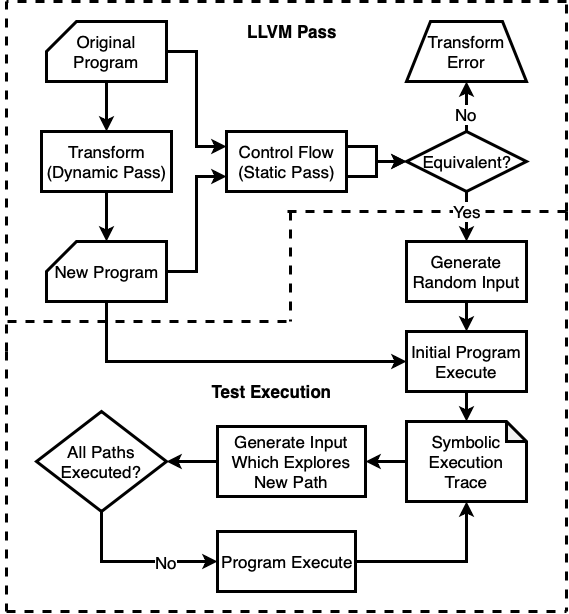
\includegraphics[width=\linewidth]{./images/overview.png}
 \caption{The general overview of our approach. Our approach starts by using LLVM's pass infrastructure to instrument the original program. We then execute the program using the symbolic execution trace to generate new inputs which drive the program on new paths.}
 \label{fig:attributes}
\end{figure}

\subsection{Dynamic Instrumentation Pass}
\label{sec:dynamic}

Our program transformation works as described in Algorithm~\ref{alg:dynamic_overview}. The algorithm takes an input $P$ which is the original program we want to run concolic testing on. The algorithm outputs $P'$: a new program which has been instrumented to output symbolic constraints of each predicate, the current variable values in each predicate and, whether the predicate final evaluation. The goal is transform $P$ to $P'$ while ensuring the control flow and decision points of both $P$ and $P'$ are equivalent.


\begin{algorithm}[t]
    \SetAlgoLined
    \SetKwProg{Fn}{Function}{}{}
    \SetKwFunction{overview}{General Overview}
    \SetKwInOut{KwIn}{Input}
    \SetKwInOut{KwOut}{Output}
    \KwIn{P}
    \KwOut{P'}

    about\_to\_branch = False\;
    P' = P\;

    \For {Each F in P}
    {
        \For {Each BB in P}
        {
            \For {Each I in P}
            {
                \If{I == Load\_Instruction}
                {
                    LHS = I.get\_LHS()\;
                    RHS = I.get\_RHS()\;
                    match\_vector = (LHS, RHS)\;
                }
                \If{I == Compare\_Instruction}
                {
                    op = I.get\_operands()\;
                    op\_m = match\_operands(op, match\_vector)\;
                    P'.log\_before(I, op\_m)\;
                    about\_to\_branch = True\;
                }
                \If{I == Branch\_Instruction}
                {
                    \If{about\_to\_branch}
                    {
                        about\_to\_branch = False\;
                        eval = evaluate\_results(I)\;
                        P'.log\_before(I, eval)\;
                    }
                }
            }
        }
    }
    
    return P'
 \caption{Dynamic Pass General Overview}
 \label{alg:dynamic_overview}
\end{algorithm}

Algorithm~\ref{alg:dynamic_overview} is an LLVM transformation pass. It works by first iterating through all functions $F$, then through all basic blocks $BB$ and then through all instructions $I$, shown in lines 3, 4 and 5 respectively. We then determine the type of instruction and handle each instruction differently. We are mainly interested in three instruction types namely, the load instruction, a compare instructions and a branch instruction as these instructions are used during program branching. The load instruction is important as it allows us to keep track of how local variables are transferred. The compare instruction compares two local variables, which determine the resulting flow of the program. Thus we are interested in obtaining the symbolic constraints from each of these compare instructions. The final instruction is the branch instruction. These instructions are where the branching actually occur in the program and thus an easy way to determine the result of a compare instruction is to evaluate the input to a branch instruction.  

Algorithm~\ref{alg:dynamic_overview} checks for a load instruction in line 6. If the instruction is indeed a load instruction the algorithm extracts the left hand side (LHS) in line 7 and right hand side (RHS) in line 8 from the instruction. The local variable in the RHS is being loaded into the local variable in the LHS. Thus we create a vector in line 9 which maps address and variables names of both sides. This mapping is used later during the constraints generation to determine which local variables are being used in each of the comparisons.

The next instruction Algorithm~\ref{alg:dynamic_overview} checks for is a compare instruction in line 11. The algorithm starts by getting the operands for the compare instruction in line 12. Using the load instructions vector, each of the operands are mapped to a known variable in line 13. Each of the operands are pass as arguments to a logging function which will display their values during a programs execution. Thus when a program is executed the constraints for each decision point in the program are printed out. Finally, line 15 sets a variable stating that a branch instruction is about to occur to true. 

The final instruction which is considered by the algorithm is a branch instruction as seen in line 17. The algorithm is only interested in branches which occur due to decision points such as compares. Other branch instructions are sometimes inserted into a program for instance to call a function. These do not change the flow of the program and so are ignored. Line 19 sets the $about\_to\_branch$ variable to false as the algorithm has found the expected branch instruction. Line 20 evaluates the result of the branch instruction. The result of this branch instruction is also the results of the compare instruction earlier. Finally algorithm~\ref{alg:dynamic_overview} prints the result of the branch instruction just before the branch occurs. Thus during execution our new program $P'$ at each decision point, we will print out the constraints containing references to known local variables and the results of each decision point will also be displayed.

\begin{algorithm}[t]
    \SetAlgoLined
    \SetKwProg{Fn}{Function}{}{}
    \SetKwFunction{overview}{General Overview}
    \SetKwInOut{KwIn}{Input}
    \KwIn{P}

    \For {Each F in P}
    {
        \For {Each BB in P}
        {
            \For {Each I in P}
            {
                \If{I == Load\_Instruction}
                {
                    LHS = I.get\_LHS()\;
                    RHS = I.get\_RHS()\;
                    match\_vector = (LHS, RHS)\;
                }
                \If{I == Compare\_Instruction}
                {
                    op = I.get\_operands()\;
                    op\_m = match\_operands(op, match\_vector)\;
                    op\_str = op\_m.to\_str()\;
                    display(op\_str)\;
                }
            }
        }
    }
 \caption{Static Pass General Overview}
 \label{alg:static_overview}
\end{algorithm}

\subsection{Static Pass}
\label{sec:static}

The static pass used an algorithm similar to the dynamic pass and is described in Algorithm~\ref{alg:static_overview}. There were however two major differences between the dynamic pass and that static pass. The first was that the static pass did not consider branching instructions. That is because the result of branching instructions can only be determined at runtime and thus is not applicable to a static pass. The second major difference is that the constraints are converted to a string representation in the static pass and displayed to the user. Thus no evaluation of the constraints takes place when the pass is run.


\subsection{Test Execution}

The process of generating and executing tests is described in Algorithm ~\ref{alg:input_testing}. To begin executing paths of the program, we first generate $n$ random values, one for each of the augmented program $P'$'s inputs as seen in lines 2 and 3. Next we create a list which will contain all the symbolic constraints found during program execution in line 5. While we have an input, $P'$ is run with these random inputs in lines 6 and 7. The program execution in line 7 returns a trace containing symbolic constraints for that specific run. This trace is appended to the list of constraints for all runs in line 8. Using the programs current trace and list of previous traces, we call a function solveConstraints which generates an input that will explore a new path in the program. Using this new input, we repeat the process until all paths have been found.

The function \textit{solveConstraints} in line 11 of Algorithm~\ref{alg:input_testing} is described as follows. First line 12 sets the input to NULL. If the constraints can not be solved this value will be returned and the concolic testing ended.  For each of the constraints in the program trace, we negate that constraint in line 14 by removing the last constraint, negating it and adding it back. If the new constraints have not been seen before, we pass them to an SMT solver which solves them and generates a new input, as shown in line 16. 

\begin{algorithm}[t]
    \SetAlgoLined
    \SetKwProg{Fn}{Function}{}{}
    \SetKwFunction{overview}{General Overview}
    \SetKwInOut{KwIn}{Input, n}
    \KwIn{P'}
    I = []\;
    \For{n times}{
        I[n] = random\_value()\;
    }
    constraints = []\;
    \While {I is not NULL}
    {
        trace = P'(I)\;
        constraints.append(trace)\;
        I = solveConstraints(trace, constraints)\;
    }
    
    \Fn{solveConstraints(T, SC)}{
        I' = NULL\;
        \For {Each t in size(T)}
        {
            new\_constraints = T - T[size(T)-t] + !T[size(T)-t]\;
            \If {new\_constraints not in SC}
            {
                I' = smt.solve(new\_constraints)\;
                break\;
            }
        }
        return I'\;
 }
    
 \caption{Input Testing Overview}
 \label{alg:input_testing}
\end{algorithm}


\section{Implementation}

Both the dynamic and the static pass were implemented in LLVM 7. In order to test our approaches we built LLVM from source and inserted our pass into the transforms directory of LLVM. Both passes were similar in that they iterated through instructions and identified different instruction types. In this section we will describe how each of the instructions were handled for both passes. We will also describe how the dynamic logging instructions were instrumented into the original program using LLVM. All code is available at: \url{https://github.com/hildebrandt-carl/concolic_testing}

\subsection{Inserting Logging Instructions}

The dynamic pass instrumented a program with logging functions to determine the symbolic constraints evaluated by the program, as well as their value during the program execution. Code Snippet~\ref{snip:original} shows a comparison instruction fcmp which inherits from the base comparison instruction class. We can see that it checks if the local variable $\%2$ is equivalent to the floating value $0.0$. The result of that $\%cmp$ is then used to determine if the program should branch or not.

\vspace{-0.6cm}

\begin{lstlisting}[caption={Original Branching Code}, label=snip:original]
Inst (fcmp): %cmp = fcmp oeq float %2, 0.0
Inst (br): br i1 %cmp, label %if.then, label %if.else
\end{lstlisting}


Our dynamic pass worked by inserting instructions which made calls to logging functions in a logging library we created. The logging library contained the declaration of multiple logging functions which we could use depending on the circumstances. For instance when a compare instruction was reached we printed out both the symbolic constraint, as well as each of the constraints run time values. The first step was to generate the symbolic constraint in a string presentation. This is done by taking the operands, finding if they are constant or local values, and then converting them to human readable form. The predicate is converted using an enumeration described by the LLVM predicate documentation.

We then insert the function call $@print\_string$ as seen in line 1 of Code Snippet~\ref{snip:instrumented}. We can see that $@print\_string$ takes two arguments $@0$ and $@1$ which are computed based on the $fcmps$ operands. Next we need to determine the value of both operands during the program execution. To do this we pass both operands to logging functions of the appropriate type. As we know the operands are 32 bit floating points we call the $@print\_float$ function. This function takes in a string and a 32 bit floating point value. We can see that the first call to the logging function in line 2 takes the first operand of the $fcmp$ in line 4, while the second call to the logging function prints out the second operand of the $fcmp$. These logging functions would thus print out the both the symbolic constraints as well as the runtime value of each operand.


\vspace{-0.4cm}

\begin{lstlisting}[caption={New Equivalent Instrumented Code}, label=snip:instrumented][H]
Inst (call): call void @print_string(i8*...@0, i8*...@1)
Inst (call): call void @print_float(i8*...@2, i32...%2)
Inst (call): call void @print_float(i8*...@3, i32...0.0)
Inst (fcmp): %cmp = fcmp oeq float %2, 0.0
Inst (call): call void @print_bool(i8*...@4, i1...%cmp)
Inst (br): br i1 %cmp, label %if.then, label %if.else
\end{lstlisting}

Finally in order to know the result of the compare statement in line 4 of Code Snippet~\ref{snip:instrumented}, we need to insert one final logging function. The result of the $fcmp$ is a 1 bit integer as seen in line 6. We thus call the appropriate logging function $print\_bool$ which takes in a 1 bit integer.

\subsection{Load Instruction}

The first instruction both Algorithm~\ref{alg:dynamic_overview} and \ref{alg:static_overview} consider is a load instruction\cite{loadinstruction}. Each time a load instruction was identified we kept track of which variables were being loaded into new memory locations. A typical example is shown below in Code Snippet~\ref{snip:load}. In this example you can see that a local variable $\%input$ is being loaded into another local variable $\%2$. The next instruction in line 2, a compare instruction, uses the local variable $\%2$. However, in order to print out the constraints for the compare instruction we need to know that the local variable $\%2$ is in fact $\%input$.

\vspace{-0.6cm}

\begin{lstlisting}[escapechar=@, caption={Load Instruction}, label=snip:load]
Inst (load): %2 = load i32, i32* %input, align 4
Inst (icmp): %cmp = icmp sgt i32 %2, 0
\end{lstlisting}

In order to keep track of these mappings we create a vector of pairings. Each pair consists of a memory location and a variable name. For instance in Line 1 when $\%input$ is stored into $\%2$, a mapping between the local variables name $\%input$ and the memory address of local variable $\%2$ is created. Thus when the local variable $\%2$ is used, our algorithm can search through the vector of known mappings and identify the variable name which is being used in any future instruction. Doing this allows us track of variables throughout the program.

\subsection{Compare Instruction}

Compare instructions, like the one seen line 2 of Code Snippet~\ref{snip:load}, are points in the program where local variables are compared. When compare instructions are paired with a branch instruction they create branches whose execution depends on the compare instruction result. Our technique thus needs to generate a symbolic constraint for each of the compare instructions. The LLVM pass we implemented checks if the instruction is a compare instruction\cite{compareinstruction}. We used the base compare instruction which all other compares inherit from, allowing us to keep the LLVM pass general. Our pass then iterates through each of the operands. If the operand is a constant value it is converted to either a constant integer or float depending on the type. If the operand is a local variable if a name can not be generated from the actual operand directly we search through the known local variable mappings. The final step is to determine the type of predicate which is used. We used the enum of predicates defined by LLVM to decode the predicate from an integer into a human readable string.

\subsection{Branch Instruction}

The last instruction we considered were branch instructions\cite{branchinstruction}. Branch instructions were only considered by the dynamic pass as we needed to evaluate them at runtime. Code Snippet~\ref{snip:branch} shows an example of a branch instruction. 
\vspace{-0.3cm}

\begin{lstlisting}[escapechar=@, caption={Branch Instruction}, label=snip:branch]
Inst (icmp): %2 = icmp sgt i32 %1, 0
// Print will be inserted here by logging
Inst (br): br i1 %2, label %if.then, label %if.else
\end{lstlisting}

 We can see that we are interested in the value of $\%2$, as this will determine whether the program branches or not. We are able to get the get the memory location of the local variable $\%2$ by requesting the branch condition and converting it to an LLVM value type. This type is then passed to our logging function which then inserts a print instruction inbetween lines 1 and 3. The logging function will then evaluate the value of $\%2$ at runtime.






\begin{figure*}[t]
 \centering
 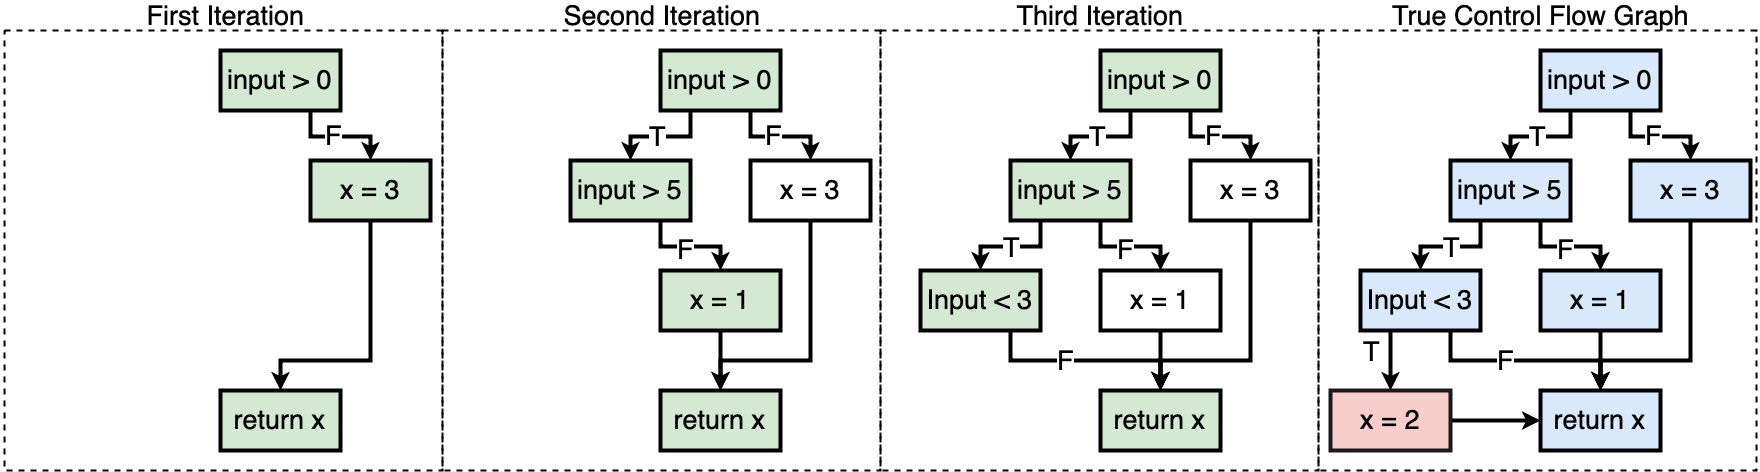
\includegraphics[width=\textwidth]{./images/cfg.png}
 \caption{The executed paths (shown in green) for each iteration of our study. The true control flow graph is depicted on the right with blue nodes depicting both nodes which our execution engine found and red nodes showing nodes which our execution engine found to be unsatisfiable.}
 \label{fig:cfg}
\end{figure*}

\section{Study}

Due to the scope of this project our main goal was to prototype this system to the point where feasibility could be shown. This study aims at showcasing this prototype while showcasing the design feasibility. The dynamic and static pass were crucial to the success of the concolic testing system. Thus both the dynamic and static LLVM pass were tested with the most common numeric data types namely:

\begin{itemize}
    \item Integers (32 bit and 64 bit)
    \item Floats (32 bit and 64 bit)
    \item Booleans (1 bit integers)
    \item Strings (8 bit integer pointers)
\end{itemize}

We also tested our LLVM passes on all of the statements which could cause branching such as if statements and loops. Interestingly, loops are handeled in the exact same way as if statements at a bitcode level. For example, consider Code Snippet~\ref{snip:loops}. The while loop was converted to an \textit{icmp} statement which is the same instruction type an if statement is converted to. Thus we later learnt that testing on both loops and if statements was actually redundant.

\vspace{-0.4cm}

\begin{lstlisting}[caption={Converting A Loop to Bit Code}, label=snip:loops]
Inst (icmp): %1 = icmp slt i32 %2, %3
Inst (br): br i1 %1, label %while.body, label %while.end
\end{lstlisting}

In order to prototype the system we implemented a constraint solver in Python using Z3. The constraint solver only handled integer values and was implemented in order to allow for a full run of the system which will discussed later in this section. 

We decided that fully automating the approach was not fundamental to showcasing the systems capabilities and thus only automated certain labour parts of the system. For instance, the process of automating the LLVM build, instrumentation, bitcode linking, and running of programs was done using shell scripts. The constraint solver was written in a single Python script and consumed trace files to automate the process of passing constraints to the solver. However in order to run a full test we manually generated traces and passed them to the solver which gave us input we manually passed back to the LLVM.

\subsection{Example Execution}

In this study, we go through an example using the program in code snippet~\ref{snip:prog}. To better understand how the execution works we also present Figure~\ref{fig:cfg} which shows which paths were executed during the concolic testing.

In our first run, we use the constraints solver to generate a random integer, which in our case was $-8361$ as seen in line 2 for Code Snippet~\ref{snip:step1}. We then run our program on this input and find that the only constraint we evaluate is $input > 0$ as seen in Code Snippet~\ref{snip:step1}. This input is evaluated as false, and there are no

\vspace{-0.6cm}

\begin{lstlisting}[caption={Original Program}, language=C, label=snip:prog]
int main(int argc, char **argv){
    int input = atoi(argv[1]);
    int x=0;
    if(input>0) {
        if(input > 5) {
            if(input < 3){
                x = 2;
            }
        }
        else{
            x = 1;
        }
    }
    else{
        x = 3;
    }
    return x;
}
\end{lstlisting}
\noindent
more predicates to evaluate on this path. Code Snippet~\ref{snip:step1} shows the system output for both the constraint solver and LLVM dynamic pass. We then pass the constraints from the LLVM trace to our constraint solver program, \texttt{solveConstraints.py}. This programs
negates the most recent un-negated constraint. In this case we negate the only constraint namely, !(input > 0). We then check if there is a satisfiable solution, which there is, and then generates new input.

\vspace{-0.6cm}

\begin{lstlisting}[caption={System Output - First Iteration}, label=snip:step1]
How many inputs values does this program take: 1
Your values are: [-8361]
=======================
Constraint Hit: input > 0
Operand (input): -8361 | Operand (0): 0
Predicate Evaluation: False
\end{lstlisting}

The new input which was generated was the value 1 as seen in line 1 of Code Snippet~\ref{snip:step2}.
On the second run, the program returns a trace saying that it evaluated two constraints upon execution, $input > 0$ as true and $input > 5$ as false. Each of these branches can be seen in the second iteration Figure~\ref{fig:cfg} as well as in the LLVM dynamic pass output in Code Snippet~\ref{snip:step2}. When we pass these constraints to our input generator, it negates $input > 5$ and generates the input of 6. 

\vspace{-0.6cm}

\begin{lstlisting}[caption={System Output - Second Iteration}, label=snip:step2]
sat - New Input: [a = 1]
========================
Constraint Hit: input > 0
Operand (input): 1 | Operand (0): 0
Predicate Evaluation: True
-----------------------
Constraint Hit: input > 5
Operand (input): 1 | Operand (5): 5
Predicate Evaluation: False
\end{lstlisting}

The third run, as seen in Code Snippet~\ref{snip:step3}, evaluates three constraints, $input > 0$ as true, $input > 5$ as true and $input < 3$ as false. We pass these constraints to our constraint solver with the last constraint, $!(input < 3)$, negated. Since input can not be both greater
than 5 and less than 3, this returns unsat. It is at this point that we have executed all paths in the control flow graph.

This ability to both stop after an unsat condition was found and consider flow senestive symbolic constraints is extremely useful. Consider for instance our static analysis LLVM pass whose results for the same original program are shown in Code Snippet~\ref{snip:static}. There is no way to tell which constraints are along the same branch, and the order in which these constraints are applied are unknown. 

\vspace{-0.6cm}

\begin{lstlisting}[caption={System Output - Final Iteration}, label=snip:step3]
sat - New Input: [a = 6]
========================
Constraint Hit: input > 0
Operand (input): 6 | Operand (0): 0
Predicate Evaluation: True
-----------------------
Constraint Hit: input > 5
Operand (input): 6 | Operand (5): 5
Predicate Evaluation: True
-----------------------
Constraint Hit: input < 3
Operand (input): 6 | Operand (3): 3
Predicate Evaluation: False
\end{lstlisting}

\vspace{-0.6cm}

\begin{lstlisting}[caption={System Output - Static Analysis}, label=snip:static]
Constraint: input > 0
Constraint: input > 5
Constraint: input < 3
\end{lstlisting}

Similarly our engines ability to determine that the constraints are unsat is extremely useful. Consider the case where path coverage is being used as a stopping condition for a random input fuzzer. The fuzzer would waste tons of execution trying to hit a branch which after only three executions of this approach was determined to be unsat.

\section{conclusion}
In this paper, we first presented and implemented a framework for doing concolic testing on LLVM bitcode. This involves two LLVM passes and a python program. The first LLVM pass
generates symbolic constraints for a program statically. The second LLVM pass inserts prints statements that generates program traces of the constraints evaluated on that
execution. These constraints are then passed to the python program which uses an SMT solver to find new inputs that satisfies new constraints of a program.

When compared against the constraints generated by the static pass, the dynamic pass along with constraint solver generate fewer inputs that still satisfy all paths. This
is due to the fact that the dynamic pass is flow sensitive unlike the static pass. If we were to generate input based solely on the static constraints, we would have to generate an
input for every satisfiable conjunction of the constraints to ensure we hit all paths. 

\bibliographystyle{ACM-Reference-Format}
\bibliography{bibliography.bib}

\end{document}
\endinput
